Photoelectron multiplier tube is one of the most used photosensors in nuclear physics during last decades. Its main objective, like all photosensors, is to detect the scintillating photons that reach its sensible part and covert it in an electronic signal large enough to be measured. 

In the figure \ref{fig:SchemePMT} we have a schematic drawing where we can see the PMT components and how it works. First of all, as we can see in the figure \ref{fig:SchemePMT}, we need to create electrons that will travel in the medium (electronic signal). To increase the amount of conserved electrons, we need to work inside a vacuum tube. Therefore, the PMT consists of a vacuum tube that has a glass window through which photons will penetrate inside. 

\begin{figure}[htbp]
\centering
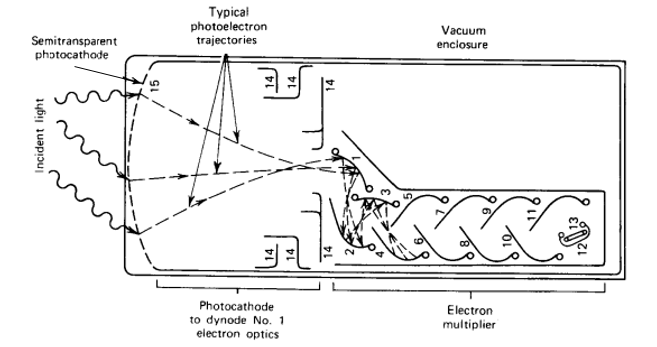
\includegraphics[scale=0.6]{3DesignPrinciples/32Tritium_detector/PMTschematic.png}
\caption{Scheme of a PMT.\label{fig:SchemePMT}~\cite{Knoll}}
\end{figure}

The way in which PMT achieves their aim of detecting scintillating photons happen inside this vacuum tube and it is based in two different phases:

\begin{itemize}
\item{} First, the PMT convert photons that reach its sensible part in electrons, called photoelectrons, with some probability through photoelectric effect. This sensitive part is the photocathode, which consists of a thin layer (thickness of the order of nanometers) deposited on the inner surface of the PMT windows. The material of the photocathode is chosen to increase the probability of producing photoelectric effect with the scintillating photons. The PMTs which we have used in this experiment are the model R8520-406 from Hammatsu \cite{DataSheetPMTs}. The material of the photocathode in our case is Bialkali.

The response of the PMT at long wavelengths is limited mainly because the photon does not have enough energy to produce a photoelectric effect or the emitted photoelectron does not have enough energy to overcome the material-vacuum interface. The response of the PMT at short wavelengths is limited mainly due to absorption in the window material, quartz in our case. Due to both reasons, the response of the PMT will have a strong dependence with the energy of the photon and it's commonly expressed in the quantum efficiency (QE) spectrum which is the quotient between the number of photoelectrons produced at the cathode of the PMT and the number of photons reaching it. For our PMTs, is showed in the figure \ref{fig:QuantumEfficiencyPMT}.

\begin{figure}[htbp]
\centering
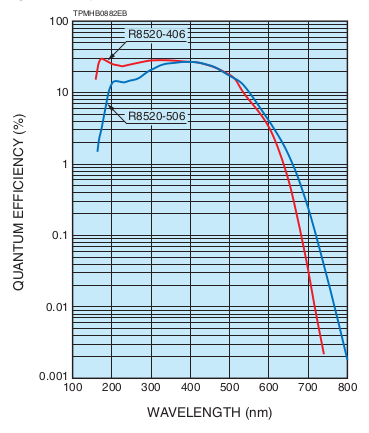
\includegraphics[scale=0.5]{3DesignPrinciples/32Tritium_detector/QuantumEfficiencyPMT.png}
\caption{Quantum efficiency spectrum for the PMT used (R8520-ZB277).\label{fig:QuantumEfficiencyPMT}~\cite{DataSheetPMTs}}
\end{figure}

The maximum values of the PMT quantum efficiency is commonly between $20\%$ and $30\%$ \cite{Knoll} (a little bit less than $30\%$ in our case \cite{DataSheetPMTs}). If we compare the emission spectrum of our scintillating fibers, figure \ref{fig:EmissionSpectrumFibers}, with the quantum efficiency spectrum of the PMTs that we have uses, figure \ref{fig:QuantumEfficiencyPMT}, we can see that the peaks of the spectrum are more or less in the same position ($435~\nm$ for the fibers and $420~\nm$ for the PMT and approximately the same value for $435~\nm$). As I said in the subsection \ref{subsec:Photosensors}, it is very important for increasing the overall efficiency of our scintillation detector. 

\item{} Next, Due to the reason that the number of photoelectrons in the photocatode is very small, we need a electron multiplication stage to achieve a large enough electronic signal to be processed by the electronic system. 

This stage is based on three elements, focusing electrodes, dynodes and anode: They are metallic sheet whose shape and position are designed to optimize the collection of the electrons. The PMT needs a high voltage (HV) which are distributed between all this elements, including the photocathode, in a increasing voltage way in order to attract and accelerate the electrons. This voltage division is achieved with an electronic circuit than can be fed with positive voltage (ground in the photocathode) or negative voltage (ground in the anode). The comercial electronic circuits of Hammatsu are showed in the figure \ref{fig:VoltageDividerCircuit}.

\begin{figure}[htbp]
\centering
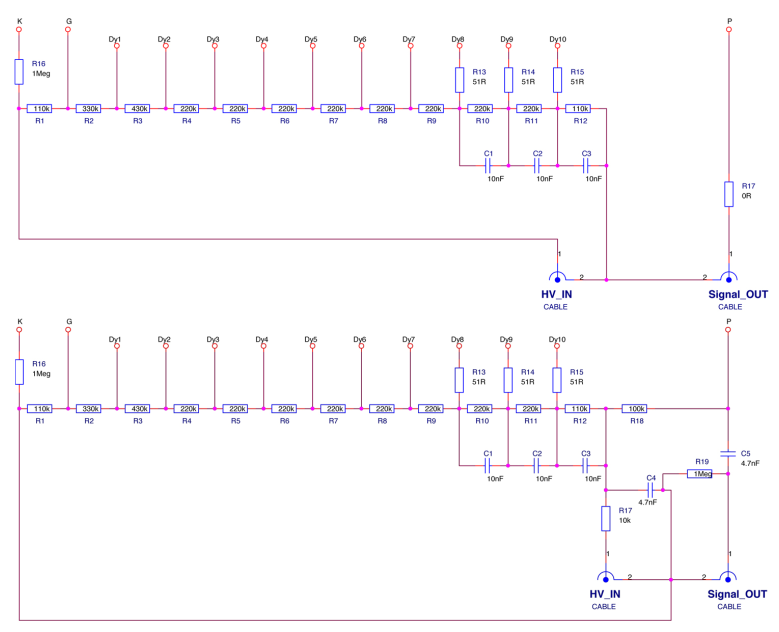
\includegraphics[scale=0.5]{3DesignPrinciples/32Tritium_detector/VoltageDividerPMT.png}
\caption{Hamamatsu commercial voltage divider electronic circuit. Upper circuit with negative supply and lower circuit with positive supply.\label{fig:VoltageDividerCircuit}~\cite{DataSheetPMTs}}
\end{figure}

The electronic circuit that can be supplied with negative voltage is faster due to the ausence of the capacitances C4 and C5, but the other circuit, supplied with positive voltage, can be interesting for other tasks such as measurement of PMT currents. We will use both, depends on the objective of the study.

Focusing electrodes are used to get the photoelectrons to reach the first dinode. Therefore, they have an collection efficiency (CE) that is defined as the quotient between the number of photoelectrons reaching the first dinode and the number of photoelectrons leaving the photocathode and whose value is around $80\%$ for PMTs.

The dynodes is the part where the multiplication takes place. They have different voltage between each dynode in order to accelerate the electrons sufficiently so that, when the electron hit the each dynode, several electrons are emitted. The multiplication factor, $\delta$, is the multiplication of electrons in each dinode and its value is commonly around 5 and it has a strongly dependence with the HV. If we take into accout that the PMT has N dynodes, commonly N=10 and we guess that each dynode has de the same gain, $\delta$, the overall gain of the PMT is:

\begin{equation}
G = CE\cdot{} \delta^N~\cite{Knoll}
\label{eq:PMTGain}
\end{equation}


If we use the numerical values mentioned in this section, we can see that the overall gain of a general PMT will be of the order of $10^6$. It is important to mention that this value depend strongly on the HV used.

We have to take into account that the uncertainty of the output signal with this gain is much greater than without it. That is the reason why, there are some times that it is interesting to work without gain such as when we try to count the number of photons that reach our PMT. We can achieve it with a small modification of the electronic voltage divider circuit \ref{fig:VoltageDividerCircuit}. It consists of short-circuiting all the dindes and the anode. In this way we are collecting the signal in the photocatode in which no amplification has occurred. We will use this voltage divider circuit without gain in our study with fibers.

Finally, when the amplification is used, the anode is the point where the collection of all the electrons produced in this multiplication process takes place and it is the one that gives rise to the output signal of PMTs. 

\end{itemize}

Due to the fact that all intermediate factors (photoelectric effect and multiplication of electrons) are linear, the output signal of a PMT will be linear with the number of photons that reach its sensitive part. It will occur until a large number of photons reach the photocathode at the same time, where saturation will occur and linearity will be lost. This limit depend on the specifically PMT which we are using. This output signal has a spread of the order of tens of nanoseconds.

The multiplication of electrons can be described as a Poisson statistical process, so, for each electron in the first dinode, we will have G new electrons whose variance will be approximately $\sqrt{G}$.

Finally, we have to take into account that the photocathode can emit electrons whose origin doesn't belong to the scintillation light. This signal, which is named dark current, can  happen due to several reasons like cosmic radiation, light from environment or thermoionic emission (the dominant) and, for our PMTs, this value will be around $2~\nano\ampere$ according to Hammamatsu data sheet.

The calibration of the most important parameters (for our objective) of the PMTs used, which are dark current, gain for several HV and quantum efficiency,  have been done at IFIC in the framework of NEXT experiment \cite{CalibrationPMTsNEXT}. 